%license:BSD-3-Clause
%copyright-holders:Michele Maione
%============================================================
%
%	Piattaforma di cloud gaming per giochi arcade
%
%============================================================

% !TeX TXS-program:compile = txs:///pdflatex/[--shell-escape]

\documentclass[openany]{book}

\usepackage[T1]{fontenc}
\usepackage[a4paper]{geometry}		% Formato del foglio
\usepackage[italian]{babel}			% Supporto per le lingue
\usepackage[utf8]{inputenc}			% Supporto per UTF-8
\usepackage[a-1b]{pdfx}				% File conforme allo standard PDF-A (obbligatorio per la consegna)
\usepackage{imakeidx}
\usepackage{float}
\usepackage{emptypage}
\usepackage{tablefootnote}
\usepackage{graphicx}				% Funzioni avanzate per le immagini
\usepackage{hologo}					% Bibtex logo with \hologo{BibTeX}
\usepackage{amssymb,amsmath,amsthm} % Simboli matematici
\usepackage{listings}				% Scrittura di codice
\usepackage{algorithm} 
\usepackage{algpseudocode} 
\usepackage{verbatim}
\usepackage{commath}
\usepackage{minted}
\usepackage{csquotes}
\usepackage{caption}

%style scritta nella bibliografia
%citestyle scritta nel testo
\usepackage[style=ext-authoryear,sorting=nty,maxbibnames=15]{biblatex}

\def\myCDL{Corso di Laurea Magistrale in Informatica}
\def\myTitle{Piattaforma di cloud gaming per giochi arcade}

\def\myName{Michele Maione}
\def\myMat{Matr. Nr. 931468}

\def\myRefereeA{Prof. Dario Maggiorini}
\def\myRefereeB{Prof. Davide Gadia}

\def\myYY{2020-2021}

\title{Piattaforma di cloud gaming per giochi arcade}
\author{Michele Maione}

\DeclareOuterCiteDelims{parencite}{\bibopenbracket}{\bibclosebracket}

\definecolor{grigio}{RGB}{100,100,100}
\captionsetup[figure]{font={footnotesize, color=grigio}}

\hypersetup{hidelinks}

\addbibresource{Bibliografia.bib}

\newcounter{savepage}

\makeindex[columns=2, title=Indice analitico]

\begin{document}
% GENERAZIONE DEL FRONTESPIZIO
\begin{titlingpage}
%\begin{titlepage}
%\pagenumbering{gobble}	

\begin{center}
	{\LARGE \uppercase{Università degli Studi di Milano}}\\
	\uppercase{Facoltà di Scienze e Tecnologie}\\
	\vskip 0.4 cm
	\uppercase{Dipartimento di Informatica\\Giovanni Degli Antoni}\\
	\vskip 0.6 cm
	\centerline{
\includegraphics[height=30mm]{immagini/unimi}}
	\vskip 0.4 cm
	\Large\uppercase{\myCDL}

	\vfill
	\vskip 1.5 cm

	{\Large\uppercase\expandafter{\myTitle}}
\end{center}

\vfill
\vskip 3 cm
		
\begin{tabular}{ll}
	{\large Relatore:} & \myRefereeA\\
	{\large Correlatore:} & \myRefereeB\\
\end{tabular}	

\vfill
\vskip 0.5 cm

\begin{flushright}
	\begin{tabular}{l}
		{\large Tesi di Laurea di:}\\
		{\large \myName}\\
		{\large \myMat}\\
	\end{tabular}	
\end{flushright}
	
\vfill
\vskip 3 cm

\begin{center}
	%inserire l'anno accademico
	%\sc anno accademico \myYY
	Anno Accademico \myYY
\end{center}

\end{titlingpage}
%\end{titlepage}

\frontmatter
{
\raggedleft \large %\sl 
	``Se non così, come? E se non ora, quando?''
	
	\bigskip
	
	\textemdash Primo Levi\\
}

\chapter*{Ringraziamenti}
Rivolgo il primo ringraziamento al prof. Dario Maggiorini per il suo continuo supporto e per avermi proposto questo progetto con la codebase di C/C++ più grande e ben strutturata che abbia mai compilato e modificato. È stata un'esperienza entusiasmante e altamente formativa.

Ringrazio il prof. Davide Gadia per la sua guida utile durante i miei sforzi verso il completamento della presente tesi.

\begin{flushright}
	Milano, luglio 2021
\end{flushright}

\addcontentsline{toc}{chapter}{Ringraziamenti}

%license:BSD-3-Clause
%copyright-holders:Michele Maione
%============================================================
%
%	Piattaforma di cloud gaming per giochi arcade
%
%============================================================

\chapter*{Sommario}
\addcontentsline{toc}{chapter}{Sommario}

%Il sommario deve contenere 3 o 4 frasi tratte dall’introduzione di cui la prima inquadra l’area dove si svolge il lavoro (eventualmente la seconda inquadra la sottoarea più specifica del lavoro), la seconda o la terza frase dovrebbe iniziare con le parole “Lo scopo della tesi è . . . ” e infine la terza o quarta frase riassume brevemente l’attività svolta, i risultati ottenuti ed eventuali valutazioni di questi.
Negli ultimi anni sono apparse molte piattaforme come Dropbox, Office 365, Netflix, Spotify, ecc\dots, che sfruttano il paradigma del cloud computing per offrire servizi accessibili su richiesta e da remoto per archiviare file, utilizzare le suite per l'ufficio, vedere film e serie TV, ascoltare musica e a partire dal 2011 anche videogiocare.

Il cloud gaming è un servizio che unisce il cloud computing e il live streaming per rendere possibile videogiocare in remoto senza scaricare o installare il gioco sul device dell'utente, in pratica consente di archiviare ed eseguire i videogiochi su un server remoto e trasmettere l'output audio-video all'utente sul proprio dispositivo.

Per far conoscere alle nuove generazioni i videogiochi che hanno fatto la storia e dare la possibilità di poter giocare ancora a macchine che ormai hanno cessato di funzionare per motivi di obsolescenza, sfruttando due tecnologie entrate a far parte della quotidianità, il live streaming e il cloud computing, in questo lavoro si propone la creazione di una piattaforma di cloud gaming. La piattaforma permetterà lo streaming audio-video, direttamente e su richiesta, dei videogiochi da un server remoto ad un client (computer, console e telefono). Il gioco è archiviato, eseguito e renderizzato su un server remoto; l'input (tastiera e gamepad) viene inviato dal client al server e lì processato. Il cloud gaming permette di iniziare a giocare immediatamente poiché il gioco è già installato sul server offrendo agli utenti un rapido accesso indipendentemente dal sistema operativo e dalle capacità hardware del client utilizzato. Infine la piattaforma, indirettamente, garantisce la gestione dei diritti digitali (DRM) per gli editori. Per questo progetto verrà ampliato il software MAME (rilasciato sotto licenza GNU-GPL) che è in grado di emulare oltre 7.000 giochi arcade, di modo che possa fungere da server di cloud gaming e comunicare con un front-end HTML, rimanendo sempre indipendente dal sistema operativo, così da rendere più agevole l’installazione di uno stand per il retro-gaming.

Nel Capitolo 1 viene introdotto il cloud gaming e fatta una panoramica dei servizi presenti sul mercato; nel Capitolo 2 viene presentata l'architettura del sistema, mentre si descrivono le tecnologie utilizzate e le funzionalità create nel Capitolo 3. All’interno del Capitolo 4 vengono illustrati i risultati ottenuti. Nell'ultimo capitolo sono riportate le conclusioni finali e una lista di possibili sviluppi futuri.

\newpage
\setcounter{tocdepth}{2}
\tableofcontents

%license:BSD-3-Clause
%copyright-holders:Michele Maione
%============================================================
%
%	Piattaforma di cloud gaming per giochi arcade
%
%============================================================

\chapter*{Introduzione}
\addcontentsline{toc}{chapter}{Introduzione}
\markboth{}{INTRODUZIONE}

%L'introduzione deve essere atomica, quindi non deve contenere nè sottosezioni nè paragrafi nè altro. Il titolo, il sommario e l'introduzione devono sembrare delle scatole cinesi, nel senso che lette in quest'ordine devono progressivamente svelare informazioni sul contenuto per incatenare l'attenzione del lettore e indurlo a leggere l'opera fino in fondo. L'introduzione deve essere tripartita, non graficamente ma logicamente:
%Il capitolo che apre questa tesi



%Inquadramento generale
%La prima parte contiene una frase che spiega l'area generale dove si svolge il lavoro; una che spiega la sottoarea più specifica dove si svolge il lavoro e la terza, che dovrebbe cominciare con le seguenti parole "lo scopo della tesi è \dots", illustra l'obbiettivo del lavoro. Poi vi devono essere una o due frasi che contengano una breve spiegazione di cosa e come è stato fatto, delle attività sperimentali, dei risultati ottenuti con una valutazione e degli sviluppi futuri. La prima parte deve essere circa una facciata e mezza o due

Nel 1972 la società Atari pubblicava il primo videogioco della storia, Pong, vendendo 19.000 cabinati e presto molte altre società seguirono l'esempio. Alla fine del decennio iniziò l'epoca d'oro dei videogiochi arcade e la nascita delle console \parencite{High_Score}. I videogiochi uniscono narrativa, animazione e musica all'interattività, ed è grazie a quest'ultima che riescono ad esercitare un potenziale d'immersione e attrazione che gli altri media non hanno, tanto da diventare un fenomeno culturale di massa con centinaia di milioni di persone che giocano regolarmente ogni giorno, rendendoli attori dominanti nel settore dell'intrattenimento. L'importanza economica dei videogiochi arcade, negli ultimi vent'anni, è notevolmente diminuita a favore dei videogiochi per personal computer, console e più recentemente per mobile.

Il cloud computing è un paradigma a cui siamo ormai abituati e ci risulterebbe difficile abbandonare servizi come Dropbox, Office 365, Spotify e Netflix per tornare alle loro versioni "precedenti": i rullini fotografici, i documenti aziendali negli archivi, i CD audio ed i DVD a noleggio. Dalla nascita dei primi servizi di cloud computing nel 2006 alcuni oggetti sono stati sostituiti con la loro controparte informatica portando al fallimento di aziende storiche come Blockbuster (nel 2013), Kodak (nel 2012) e Borders\footnote{Borders Group era un rivenditore americano di libri e musica.} (nel 2011) \parencite{I_4_fallimenti_più_clamorosi_del_decennio}. Il cloud computing consiste nella distribuzione on-demand delle risorse IT tramite internet su tre livelli di servizio che sono: l'accesso all'infrastruttura hardware tramite API (IaaS), la piattaforma software inclusa di sistemi di sviluppo (PaaS) e le applicazioni (SaaS). Con il cloud computing la potenza della macchina, sia essa fisica o virtuale, aumenta automaticamente all'esigenza permettendo di gestire i picchi di utilizzo; svincola gli utenti dal dover acquistare, manutenere e gestire fisicamente le infrastrutture IT; fornisce l'accesso alle risorse informatiche da qualsiasi device, da qualsiasi luogo e in modo collaborativo.

Unendo il paradigma del cloud computing con lo streaming nasce un nuovo tipo di servizio dedicato ai videogiochi: il cloud gaming. Questo servizio rende possibile videogiocare in remoto senza scaricare o installare il gioco sul device dell'utente. Con il cloud gaming i videogiochi sono archiviati ed eseguiti su un server remoto e l'output audio-video trasmesso al dispositivo dell'utente, permettendo di iniziare a giocare immediatamente, indipendentemente dal sistema operativo e dalle capacità hardware del dispositivo utilizzato. Infine, indirettamente, viene garantita la gestione dei diritti digitali (DRM) per gli editori. Il cloud gaming è l'unione di due modelli del cloud computing: il modello SaaS e il modello PaaS sia perché il videogioco viene offerto al giocatore come "applicazione" sia perché allo sviluppatore viene offerto il sistema operativo e i vari SDK, questo paradigma implementato dal cloud gaming è definito "gioco come servizio" (GaaS) che si divide in tre instanze: rendering remoto (RR-GaaS), rendering locale (LR-GaaS), allocazione delle risorse cognitive (CRA-GaaS) \parencite{Cloud_for_Gaming}.

%Breve descrizione del lavoro
%La seconda parte deve essere una esplosione della prima e deve quindi mostrare in maniera più esplicita l'area dove si svolge il lavoro, le fonti bibliografiche più importanti su cui si fonda il lavoro in maniera sintetica (una pagina) evidenziando i lavori in letteratura che presentano attinenza con il lavoro affrontato in modo da mostrare da dove e perchè è sorta la tematica di studio. Poi si mostrano esplicitamente le realizzazioni, le direttive future di ricerca, quali sono i problemi aperti e quali quelli affrontati e si ripete lo scopo della tesi. Questa parte deve essere piena (ma non grondante come la sezione due) di citazioni bibliografiche e deve essere lunga circa 4 facciate.

Lo scopo di questa tesi è creare una piattaforma di cloud gaming per far conoscere alle nuove generazioni i videogiochi che hanno fatto la storia e dare la possibilità di poter giocare ancora a macchine che ormai hanno cessato di funzionare per motivi di obsolescenza. Per far ciò verrà ampliato il software MAME (rilasciato sotto licenza GNU-GPL) che è in grado di emulare oltre 7.000 giochi arcade, di modo che possa fungere da server di cloud gaming e comunicare con un front-end HTML, rimanendo sempre indipendente dal sistema operativo, rendendo più agevole l’installazione di uno stand per il retro-gaming. 

Per la realizzazione del progetto sono state prese in considerazione le analisi fatte sulle piattaforme delle multinazionali come GeForce Now, Stadia e PlayStation Now in \parencite{A_Network_Analysis_on_Cloud_Gaming_Stadia_GeForce_Now_and_PSNow} e \parencite{Network_Analysis_of_the_Sony_Remote_Play_System}, come Amazon Luna in \parencite{Amazon_Luna_WebRTC}, ma anche progetti open source come "Games on Demand" di \parencite{ARealTimeStreamingGamesonDemandSystem} che propongono una piattaforma basata sul hooking di funzioni DirectX, codifica in MPEG2 e trasmissione tramite UDP; "GamingAnywhere" di \parencite{GamingAnywhere} che è un progetto multipiattaforma che trasmette tramite protocollo RTP e la cattura audio-video avviene utilizzando la libreria SDL tramite polling.

Il sistema proposto è stato progettato con un'ottica incentrata sull'utilizzo in LAN con l'utenza connessa tramite WiFi, ad esempio in stand di retro-gaming ad eventi di informatica e videogiochi, in aziende come servizio di svago per i clienti in sala d'attesa e per i dipendenti durante la pausa, ecc\dots, è importante ricordare che i videogiochi, nonostante siano stati pensati come fonte d'intrattenimento, migliorano diversi tipi di abilità chiave: abilità sociali e intellettuali, riflessi e concentrazione \parencite{Use_of_Cloud_Gaming_in_Education}; per questo motivo la piattaforma può essere installata anche nelle scuole.

Per ampliare il progetto MAME, lato server ho modificato le funzionalità di rendering video e missaggio audio per convogliare il loro output, che viene codificato in MPEG-TS, ad un modulo che esegue lo streaming tramite il protocollo WebSocket ad una pagina HTML. Lato client ho creato un modulo JavaScript per gestire l'input utente e decodificare il filmato MPEG-TS. La piattaforma utilizza un bit-rate tra 0.5 Mbps e 2.2 Mbps ed offre una risoluzione di 480p; per valutarne la latenza è stata testata su rete locale e su rete internet \parencite{Latency_analysis_for_M2M}; mentre la qualità audio-video è stata classificata tramite "peek signal-to-noise ratio" e "structural similarity index method" \parencite{Cloud_Gaming_Architecture_and_Performance}.



%Struttura della tesi
%La terza parte contiene la descrizione della struttura della tesi ed è organizzata nel modo seguente.
%La tesi è strutturata nel modo seguente:
%Nella sezione due si mostra \dots
%Nella sez. tre si illustra \dots
%Nella sez. quattro si descrive \dots
%Nelle conclusioni si riassumono gli scopi, le valutazioni di questi e le prospettive future \dots
%Nell'appendice A si riporta \dots (Dopo ogni sezione o appendice ci vuole un punto).
%I titoli delle sezioni da 2 a M-1 sono indicativi, ma bisogna cercare di mantenere un significato equipollente nel caso si vogliano cambiare. Queste sezioni possono contenere eventuali sottosezioni.

La tesi è strutturata nel modo seguente:
\begin{itemize}
	\item Il capitolo 1 fornisce un'introduzione sulla nascita dei videogiochi e dei ricavi globali dell'industria videoludica, dà una definizione di cloud computing e di cloud gaming, fà una panoramica delle piattaforme di gioco che si sono susseguite nel tempo e delle proiezioni di mercato del settore del cloud gaming.
	\item Nel capitolo 2 verrà descritto il sistema proposto, il MAME e le sue funzioni di: rendering, missaggio audio e gestione dell'input utente.
	\item Nel capitolo 3 verranno descritte le cinque fasi aggiuntive del cloud gaming e la loro implementazione in C++ come nuovi moduli del MAME: la cattura audio-video, la codifica, la trasmissione, la decodifica e la gestione dell'input utente.
	\item Il capitolo 4 analizza le prestazioni del progetto relativamente ai tre difetti intrinseci del cloud gaming: riduzione della qualità audio-video, bit-rate richiesto e il problema della latenza.
	\item Nelle conclusioni si riassumono gli scopi, le valutazioni di questi e le prospettive future.
	\item Nell'appendice A si riporta la documentazione del progetto logico. Il listato con l’autodocumentazione relativa è riportato nell'appendice B. Infine nell'appendice C si trova il manuale utente.
\end{itemize}

\newpage
\setcounter{savepage}{\arabic{page}}

\mainmatter
%license:BSD-3-Clause
%copyright-holders:Michele Maione
%============================================================
%
%	Piattaforma di cloud gaming per giochi arcade
%
%============================================================

\chapter{Introduzione}
\label{cap:Introduzione}

Il capitolo che apre questa tesi fa un'introduzione sulla nascita dei videogiochi, i ricavi globali dell'industria videoludica, il cloud gaming e i servizi presenti sul mercato.

\section{Nascita dei videogiochi}

Nel 1952 nei laboratori dell'Università di Cambridge, come esempio a corredo di una tesi di dottorato, fu creato OXO, la trasposizione del tris come gioco per computer. OXO è considerato tecnicamente il primo videogioco. Nel 1958 un professore di fisica del Brookhaven National Laboratory creò un gioco, Tennis for Two, che aveva il compito di simulare le leggi fisiche relative ad una partita di tennis, lo strumento utilizzato era un oscilloscopio.

Nel 1961, sei giovani scienziati del Massachusetts Institute of Technology su un PDP-1\footnote{PDP-1: Programmed Data Processor-1, era un computer della Digital Equipment Corporation del 1959.} crearono il primo videogioco a scopo di intrattenimento: Spacewar!.

Due mesi dopo due ingegneri elettrici, N. Bushnell e T. Dabney, terminarono la loro versione di Spacewar! su larga scala (1.500 copie), ma il gioco non ebbe un grande successo a causa dell'elevata difficoltà. Bushnell, dopo l'esperimento non particolarmente riuscito, decise però di insistere nel settore dando così vita alla società Atari. Il primo gioco arcade di Atari fu il primo grande successo del settore: Pong. Pubblicato alla fine del 1972, è un gioco che riproduce approssimativamente la meccanica del ping pong. Atari vendette 19.000 cabinati di Pong e presto molte altre società seguirono l'esempio. Alla fine del decennio iniziò l'epoca d'oro dei videogiochi arcade.

I videogiochi sono un mezzo di intrattenimento unico che combina le diverse forme d'arte, quali musica, narrativa e animazione, all'interattività. Ed è proprio questa caratteristica, l'interattività, che permette loro di esercitare un potenziale d'immersione e attrazione che altri media non hanno. Sono ormai diventati un fenomeno culturale di massa con centinaia di milioni di persone che giocano regolarmente ogni giorno, il che li rende un attore dominante nel settore dell'intrattenimento, settore in continua crescita che non ha mai subito interruzioni nel corso degli anni come mostrato in Fig. \ref{fig:valore_commerciale_giochi_globale}. Negli ultimi vent'anni l'importanza economica dei videogiochi arcade è notevolmente diminuita\footnote{Giappone, Cina e Corea mantengono una forte industria arcade ai giorni nostri.} (in viola nella figura) a favore dei videogiochi per personal computer, console e più recentemente per mobile.

\begin{figure}[H]
	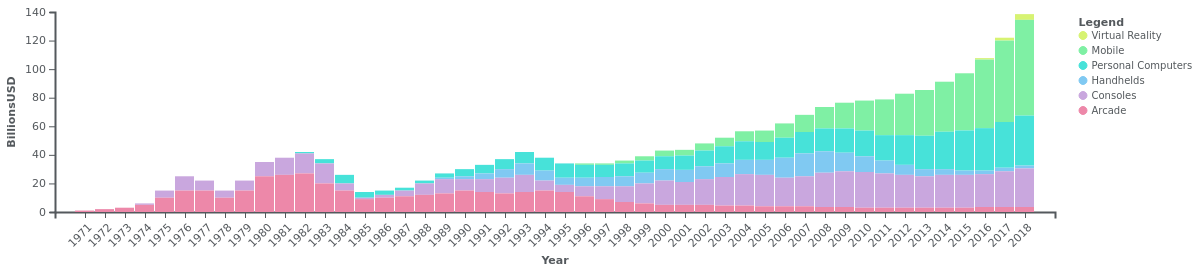
\includegraphics[width=\linewidth]{immagini/valore_commerciale_giochi_globale.png}
	\caption{Ricavi globali dell'industria dei videogiochi dal 1971 al 2018 (non adeguati all'inflazione). Fonte: wikipedia.org}
	\label{fig:valore_commerciale_giochi_globale}
\end{figure}

%\begin{figure}[H]
%	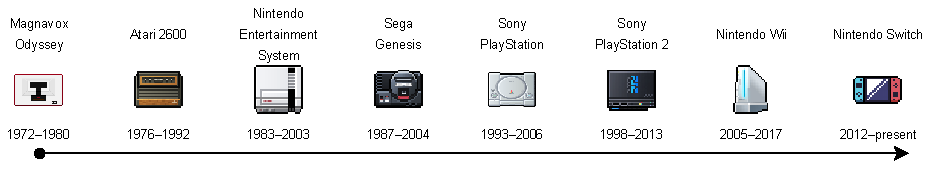
\includegraphics[width=\linewidth]{immagini/consoles_history}
%	\caption{Console iconiche, fino alla generazione otto}
%	\label{fig:consoles_history}
%\end{figure}

\section{Cloud gaming}
Il cloud gaming è un tipo di servizio online che funziona in modo simile al desktop remoto e al video on demand. I videogiochi vengono archiviati ed eseguiti in remoto, audio e video vengono trasmessi in streaming come un film sul dispositivo dell'utente, tramite un client. Il client gestisce gli input del giocatore, che vengono inviati al server ed eseguiti nel gioco.

Questo tipo di approccio offre molti vantaggi, tra cui: rende il gioco facilmente accessibile senza doverlo scaricare e installare localmente, è compatibile con computer e smartphone e anche con smart TV se utilizzato con un gamepad WiFi. Diversi servizi possono offrire alcune funzionalità aggiuntive per sfruttare al meglio questo modello, uno spettatore può unirsi alla sessione di un giocatore e assumere temporaneamente il controllo del gioco, se autorizzato dal giocatore stesso. Inoltre risolve definitivamente un problema che esiste dai tempi delle audiocassette e dei floppy disk: la pirateria. Il rapido sviluppo delle reti a banda larga e il continuo calo dei costi di abbonamento hanno reso questo metodo, oggi, una realtà.

Il più grande problema del cloud gaming era ed è ancora la latenza. Le fasi di un videogioco sono: ricezione input, esecuzione, rendering, display; mentre nel caso del cloud gaming abbiamo: ricezione input, invio input tramite rete, esecuzione, rendering, codifica, invio codifica tramite rete, decodifica, display. Una tempistica di esempio è visibile in Fig. \ref{fig:latenzaCloudGaming}. Un leggero ritardo in un filmato su internet o in una videochiamata molto probabilmente passa inosservato, ma durante una partita la latenza può rendere il gioco ingiocabile.

\begin{figure}[H]
	\includegraphics[width=\linewidth]{immagini/latenzaCloudGaming.png}
	\caption{Latenza del videogioco: locale vs cloud gaming. Fonte: shadow.tech/blog/news/roadmap-cloud-gaming-without-latency}
	\label{fig:latenzaCloudGaming}
\end{figure}

\subsubsection{La nascita del cloud gaming}
I primi accenni al cloud gaming per il grande pubblico sono arrivati solo intorno al 2010. Una delle prime piattaforme create per consentire ai giocatori di tutto il mondo di provare l'emozione del gaming in streaming è stata OnLive di OL2, presentato alla GDC\footnote{GDC: Game Developers Conference, una conferenza annuale per gli sviluppatori di videogiochi.} 2009 e poi lanciato sul mercato nel giugno 2010. I giocatori potevano acquistare giochi sulla piattaforma o giocare dalla loro libreria digitale Steam\footnote{Steam è un servizio di distribuzione digitale di videogiochi della società Valve.}.

Nel 2012, Gaikai ha inaugurato il suo servizio di cloud gaming, la società si è concentrata principalmente sull'utilizzo del cloud gaming come forma di pubblicità online per i videogiochi, dove gli utenti avrebbero avuto la possibilità di accedere alle demo dei videogiochi.

OnLive e Gaikai sono stati acquisiti da Sony e le loro risorse sono state utilizzate come base per un servizio di cloud gaming noto come Playstation Now.

Nel 2013, Nvidia ha introdotto GeForce Now, un servizio di cloud gaming integrato nel suo dispositivo Shield TV\footnote{Nvidia Shield TV è un lettore multimediale digitale basato su Android TV prodotto da Nvidia.} Dispositivo. Nel 2017, la società ha iniziato a espandere il proprio servizio su PC, incluso il supporto per l'importazione della libreria Steam di un utente.

Nel maggio 2018, Electronic Arts ha acquisito alcune risorse di cloud gaming da GameFly. EA\footnote{EA: Electronic Arts.} ha annunciato Project Atlas, un progetto che esplorava l'integrazione di intelligenza artificiale e apprendimento automatico, rendendo la piattaforma dinamica, social e multipiattaforma.

Microsoft all'E3\footnote{E3: Electronic Entertainment Expo, un evento commerciale per l'industria dei videogiochi.} del 2018 ha annunciato la sua piattaforma Xbox Cloud Gaming.

Alla GDC 2019, Google ha annunciato ufficialmente il suo servizio di cloud gaming Stadia, in uscita per novembre dello stesso anno.

A settembre 2020, un nuovo servizio chiamato Luna è stato annunciato da Amazon\cite{Cloud_gaming_history}.

\subsubsection{Apple's controversy}
Apple aveva cercato di bloccare le app di cloud gaming sul suo servizio a metà del 2020 su piattaforma iOS, ma a settembre 2020 ha modificato le sue regole che consentivano il cloud gaming con le restrizioni che i giochi offerti nel servizio devono essere scaricati direttamente dall'App Store, non da un'app all-in-one. I produttori di app sono autorizzati a rilasciare una cosiddetta "app catalogo" che si collega ad altri giochi nel servizio, ma ogni gioco dovrà essere una singola app e tutti i giochi e i negozi devono offrire l'acquisto in-app utilizzando l'app Apple. sistema di elaborazione dei pagamenti, in base al quale Apple di solito prende il 30\% delle entrate\cite{Apple_controversy}.

\subsubsection{Cloud gaming market}
Secondo la ricerca di Newzoo sull'industria dei videogiochi, nel 2020 sono stati generati quasi \$585 milioni di entrate dal mercato del cloud gaming ed è destinato a crescere notevolmente fino a \$4,8 miliardi entro il 2023. Oltre a ciò, la proiezione attuale suggerisce addirittura crescita maggiore. Per questo sono entrate nel mercato anche aziende che non sono produttori di videogiochi, come Google e Amazon.

\begin{figure}[H]
	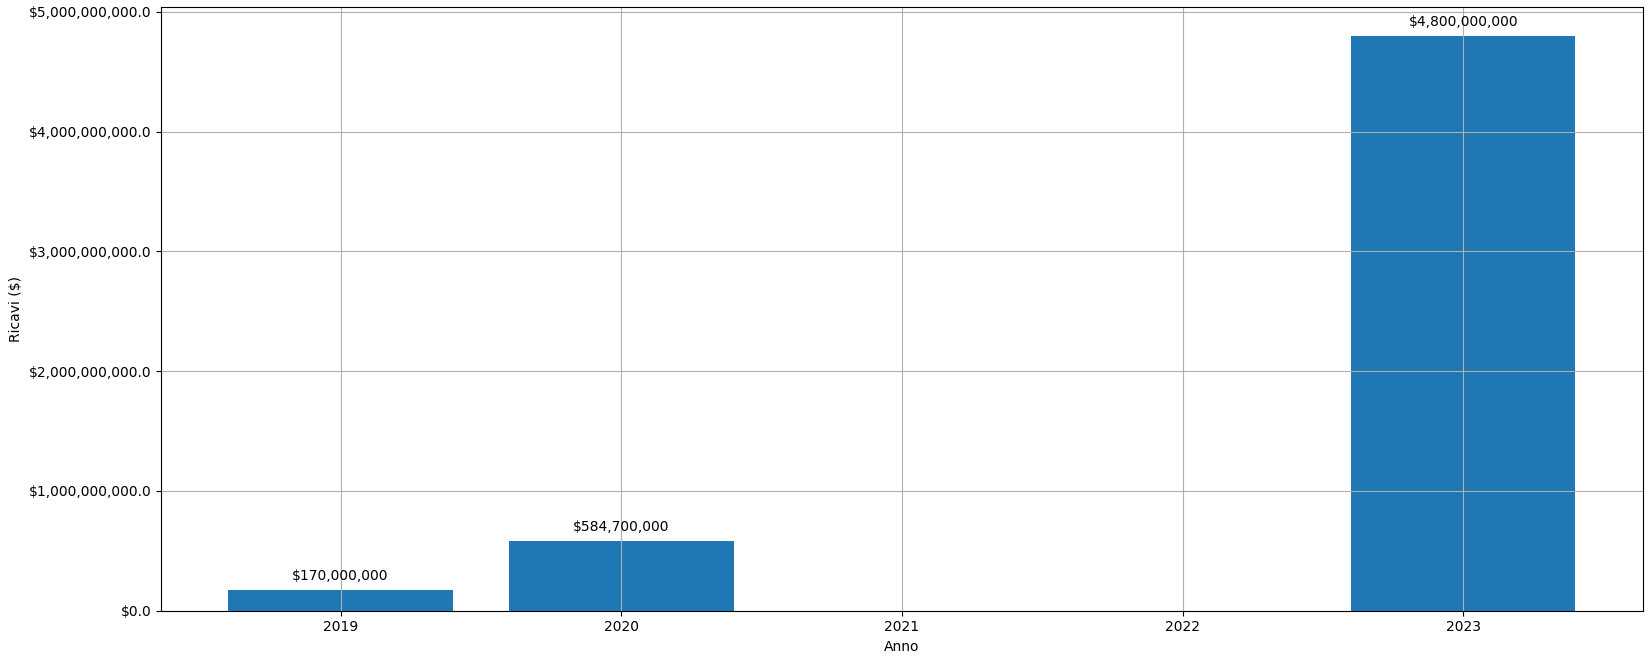
\includegraphics[width=\linewidth]{immagini/Newzoo_Cloud_Gaming_Revenues}
	\caption{Previsioni sulla capitalizzazione di mercato globale del cloud gaming in dollari americani. Fonte: newzoo.com/global-cloud-gaming-report}
	\label{fig:Newzoo_Cloud_Gaming_Revenues_Sept_2020}
\end{figure}

Vediamo l'attuale panorama del cloud gaming.

\subsection{Utomik}
La piattaforma Utomik è stata lanciata commercialmente nel 2008 e da allora è in servizio. I giochi per essere riprodotti in un browser richiedono il plug-in proprietario Utomik Player. La piattaforma offre un SDK\footnote{SDK: kit di sviluppo software, una raccolta di strumenti di sviluppo software.}, Plug-in e servizio online per creare, avviare, mantenere e monitorare i giochi \cite{Utomik}.

\subsection{Microsoft - Xbox Cloud Gaming}
Microsoft ha anticipato il servizio all'E3 2018. Il servizio è disponibile per gli abbonati a Xbox Game Pass Ultimate dal 15 settembre 2020. La piattaforma offre la libreria esistente di giochi Xbox e aggiunge nuovi giochi da Xbox Series X. Il servizio è progettato per funzionare con i telefoni (attualmente solo Android), con controlli touchscreen o controller Xbox tramite Bluetooth\cite{Xbox_Game_Pass_cloud_gaming}.

\subsection{Project Atlas}
A maggio 2018 Electronic Arts ha svelato la sua piattaforma di gioco nativa per il cloud chiamata Project Atlas, che mira a rendere disponibili numerosi titoli giocabili attraverso i server dell'azienda ea fornire un'esperienza di gioco mai provata prima grazie al supporto dell'intelligenza artificiale. La piattaforma intende offrire un'esperienza di cloud gaming composta da universi realmente viventi, che cambiano con il passare del tempo, con l'interazione con altri giocatori e sotto l'influenza del mondo esterno. In questi processi, il supporto dell'intelligenza artificiale e l'apprendimento delle abitudini e delle preferenze dei giocatori giocherebbero un ruolo fondamentale. Offre anche un client di gioco dinamico, che consente agli utenti di riprodurre in streaming un titolo mentre attendono il completamento del download sul disco di archiviazione del proprio dispositivo\cite{Project_Atlas}.

\subsection{Nvidia - GeForce Now}
GeForce Now è il servizio di cloud gaming di Nvidia lanciato in beta a gennaio 2017 e ufficialmente a febbraio 2020. GeForce Now consente agli utenti di accedere da remoto (tramite streaming) a un computer virtuale, dove possono installare i giochi acquistati su Steam, Ubisoft Connect\footnote{Ubisoft Connect è un servizio di distribuzione digitale, gestione dei diritti digitali, multiplayer e comunicazione sviluppato da Ubisoft.} O Epic Games Store\footnote{Epic Games Store è un negozio di videogiochi digitali gestito da Epic Games.}. Il servizio può essere utilizzato su Windows, macOS, iOS, Android o Nvidia Shield TV\cite{GeForce_Now}.

\subsection{Sony - PlayStation Now}
PlayStation Now è un servizio di abbonamento al cloud gaming basato sulla tecnologia cloud di Gaikai e Microsoft Azure. È stato presentato durante il CES\footnote{CES: Consumer Electronics Show, un evento annuale che ospita presentazioni di nuovi prodotti e tecnologie nel settore dell'elettronica di consumo.} 2014. È disponibile da gennaio 2015 in Nord America, da settembre in Giappone e Regno Unito . Il servizio ha iniziato ad operare in Europa gradualmente da agosto 2017 a marzo 2019. Il servizio consente all'utente di giocare ai titoli PlayStation (dal catalogo giochi di PS2, PS3 e PS4) su PS4, PS5 e Windows\cite{PlayStation_Now}.

\subsection{Google - Stadia}
Stadia è una piattaforma di cloud gaming rilasciata a novembre 2019, ma è disponibile solo in Europa e negli Stati Uniti. Sulla piattaforma l'utente può acquistare giochi o iscriversi al servizio per accedere al catalogo giochi.

Google ha creato il controller Stadia che si connette tramite WiFi direttamente al servizio e rende possibile giocare su una TV (installando l'app o utilizzando un Chromecast \ footnote {Google Chromecast is digital media player for Internet-streamed audiovisual content}). Puoi giocare con mouse e tastiera o controller utilizzando il browser Chrome su qualsiasi PC. È disponibile un'app mobile che supporta i controlli touch screen e i gamepad Bluetooth.

La piattaforma offre alcune funzionalità interessanti come: condividere il gameplay tramite un live streaming su YouTube; Crowd Play che consente agli spettatori di unirsi ai giochi multiplayer che stanno guardando; Stream Connect che consente all'utente di condividere la schermata di gioco con altri giocatori nello stesso gioco; Condivisione dello stato che consente ai giocatori di condividere il proprio stato di salvataggio\cite{Google_Stadia}.

\subsection{Amazon - Luna}
Luna è stata annunciata il 24 settembre 2020, con "accesso anticipato" disponibile per gli abbonati su invito a partire dal 20 ottobre 2020. Amazon Luna avrà 100 giochi diversi al lancio e sarà alimentato da AWS. Luna avrà l'integrazione con Twitch. Amazon ha stretto una partnership con Ubisoft per creare un canale di gioco (con costi aggiuntivi) esclusivo di Luna, che darà agli abbonati di Luna l'accesso ai titoli di Ubisoft lo stesso giorno in cui vengono rilasciati.\cite{Amazon_Luna}.

\subsection{RemoteMyApp - Vortex}
Il servizio è stato lanciato a novembre 2018. Il servizio è disponibile per Android, Windows e macOS, offre tre piani mensili (\$12, \$23 e \$33) che consentono all'utente di giocare per un massimo di 140 ore al mese e il catalogo è composto da 170 giochi. Sfortunatamente, alcuni giochi possono essere riprodotti solo acquistando la licenza del gioco\cite{RemoteMyApp_Vortex}.

\subsection{Playkey}
Una menzione speciale va fatta alla società Playkey, che ha realizzato una piattaforma di cloud gaming distribuita. I giocatori non si connettono a un server per ricevere lo streaming del gioco, ma al computer di un minatore, su cui viene eseguito il gioco. Non ci sono server potenti, perché ci sono computer distribuiti in tutto il mondo che fungono da server, i minatori guadagnano \$10 al giorno. I giocatori possono giocare solo dalla loro libreria di giochi personale\cite{Playkey}.
%license:BSD-3-Clause
%copyright-holders:Michele Maione
%============================================================
%
%	Piattaforma di cloud gaming per giochi arcade
%
%============================================================

\chapter{Soluzione proposta}
In questo capitolo verrà fatta\dots



\section{Sistema proposto}
L'esigenza per la quale nasce questo progetto è far conoscere alle nuove generazioni i videogiochi che hanno fatto la storia e dare la possibilità di poter giocare ancora a macchine che ormai hanno cessato di funzionare per motivi di obsolescenza, sfruttando due tecnologie entrate a far parte della quotidianità, lo streaming e il cloud computing. In questo lavoro si propone la creazione di una piattaforma di cloud gaming, che permette lo streaming audio-video direttamente e su richiesta dei videogiochi, da un server remoto, ad un client (computer, console, telefono). Per far ciò verrà ampliato il software MAME (rilasciato sotto licenza GNU-GPL) che è in grado di emulare oltre 7.000 giochi arcade. Le caratteristiche principali del progetto, che sono state vincolanti nella scelta delle tecnologie da utilizzare, sono la portabilità e la possibilità di utilizzare il sistema senza dover installare software aggiuntivi, e per questi vincoli, lato client, la scelta è ricaduta sul browser web. In Fig. \ref{fig:webprotocols} sono schematizzati i protocolli, i servizi e le API relativi alle tecnologie di streaming per i browser web ad oggi disponibili\cite{Audio_and_video_delivery}, che sono:

\begin{itemize}
	\item WebSocket è un protocollo di comunicazione che fornisce un canale full-duplex su una singola connessione TCP, con una latenza inferiore rispetto ad HLS e DASH;
	\item HTTP Live Streaming (HLS) è il protocollo di streaming ad alta latenza più popolare su HTTP per video on demand (video preregistrato) sviluppato da Apple;
	\item Dynamic Adaptive Streaming over HTTP (DASH) è una tecnica di streaming con bit-rate adattivo del Moving Picture Experts Group (MPEG), che consente lo streaming di alta qualità di contenuti multimediali su protocollo HTTP;
	\item Web Real-Time Communication (WebRTC) è un progetto per la comunicazione in tempo reale basato sul protocollo RTP (Real-time Transport Protocol)\cite{High_Performance_Browser_Networking}.
\end{itemize}

\begin{figure}[H]
	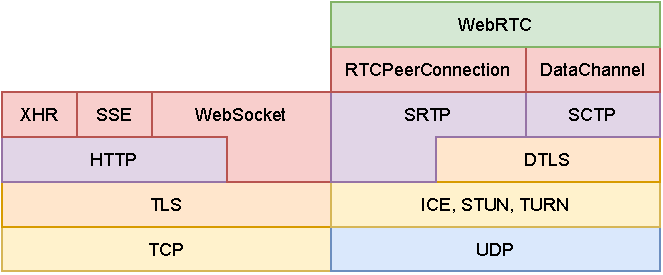
\includegraphics[width=\linewidth]{immagini/webprotocols}
	\caption{API, protocolli e servizi di rete del browser di alto livello}
	\label{fig:webprotocols}
\end{figure}

Il sistema è stato progettato con un'ottica incentrata sull'utilizzo in stand di retro-gaming ad eventi di informatica e videogiochi, da utilizzare quindi sulla rete locale dell'evento con gli utenti connessi tramite WiFi. In questo contesto la differenza di velocità tra TCP e RTP può essere trascurata, e la scelta della tecnologia di streaming da usare è ricaduta su WebSocket perché è un protocollo di comunicazione standardizzato dal 2011, è pienamente supportato da tutti i browser moderni, ha una latenza inferiore rispetto ad HLS e DASH, è semplice da instanziare e non richiede l'utilizzo di protocolli aggiuntivi o configurazioni complesse a differenza di WebRTC.

\begin{figure}[H]
	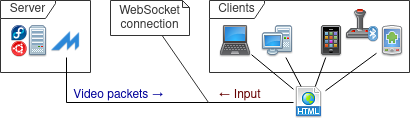
\includegraphics[width=\linewidth]{immagini/proposed_system}
	\caption{Panoramica del sistema}
	\label{fig:proposed_system}
\end{figure}

Come mostrato in Fig. \ref{fig:proposed_system} il sistema è costituito dal server di gioco, che può essere Linux, Windows o macOS, su cui è in esecuzione la versione modificata di MAME ed una pagina HTML5 che funge da front-end. Il programma è in ascolto per connessioni WebSocket con parametri (per es.: il nome del gioco, l'ID del player, l'ID della partita). Una volta stabilita la connessione, il server invia informazioni sulla dimensione e le proporzioni del video e avvia il gioco. Il rendering e il missaggio audio del gioco vengono generati utilizzando la libreria SDL\footnote{SDL: Simple DirectMedia Layer, una libreria multipiattaforma ed open-soure per il multimedia}, codificati e pacchettizzati nel contenitore MPEG-TS\footnote{MPEG-TS: MPEG transport stream, è un contenitore digitale per la trasmissione e l'archiviazione audio-video.} usando la libreria FFmpeg\footnote{FFmpeg è una suite open-source di librerie e programmi per la gestione di video, audio, e altri file multimediali e stream.} e inviati tramite WebSocket al client.

Lato client vari script si occupano di decodificare i dati audio-video ricevuti, catturare e inviare l'input dell'utente, sia dalla tastiera che dal gamepad, al server tramite WebSocket.



\section{Come funziona il MAME}
Lorem ipsum dolor sit amet, consectetur adipiscing elit, sed do eiusmod tempor incididunt ut labore et dolore magna aliqua. Ut enim ad minim veniam, quis nostrud exercitation ullamco laboris nisi ut aliquip ex ea commodo consequat. Duis aute irure dolor in reprehenderit in voluptate velit esse cillum dolore eu fugiat nulla pariatur. Excepteur sint occaecat cupidatat non proident, sunt in culpa qui officia deserunt mollit anim id est laborum.

\subsection{Simple DirectMedia Layer (SDL)}
SDL è una libreria multipiattaforma che fornisce accesso di basso livello ad audio, tastiera, mouse, gamepad, hardware 3D e framebuffer 2D. Come mostrato in Fig. \ref{fig:sdl} SDL è costruito sopra le API di visualizzazione video del sistema operativo (in arancione), librerie di rendering 3D (in verde) e librerie che si interfacciano alla scheda audio (in rosso)\cite{SDL_Wiki}.

\begin{figure}[H]
	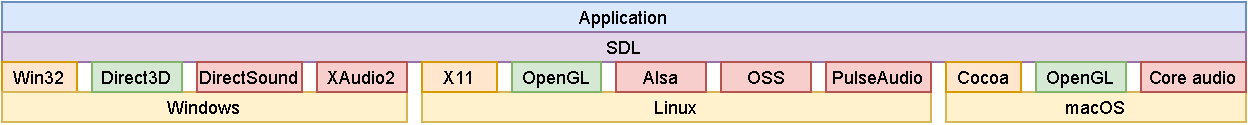
\includegraphics[width=\linewidth]{immagini/sdl}
	\caption{SDL: livelli di astrazione su diverse piattaforme}
	\label{fig:sdl}
\end{figure}

\subsection{Video}
Il MAME è in grado di emulare giochi sia 2D che 3D (es.: Tekken della Namco), ma poiché emula fisicamente il monitor del cabinato ciò che viene inviato alla libreria grafica è un insieme di primitive e texture da disegnare.

\begin{figure}[H]
	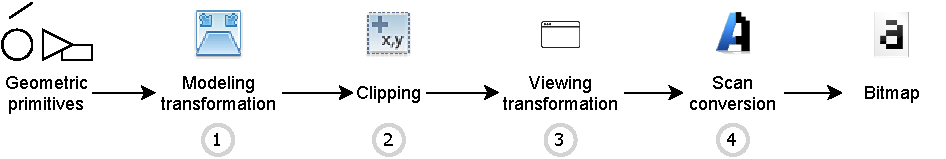
\includegraphics[width=\linewidth]{immagini/rendering_pipeline}
	\caption{Pipeline di rendering 2D}
	\label{fig:rendering_pipeline}
\end{figure}

\subsubsection{SDL renderer} \label{SDL_renderer}
Quando la finestra di gioco viene inizializzata, viene creato un contesto di rendering SDL per la finestra tramite la funzione \textit{CreateRenderer}. Per ogni frame della macchina che viene emulato c'è una fase di disegno usando \textit{SetRenderDrawColor}, \textit{RenderFillRect} e \textit{RenderDrawLine}, e poi tramite la funzione \textit{RenderPresent} viene mostrato il frame appena renderizzato sulla finestra.

\subsection{Audio}
Lorem ipsum dolor sit amet, consectetur adipiscing elit, sed do eiusmod tempor incididunt ut labore et dolore magna aliqua. Ut enim ad minim veniam, quis nostrud exercitation ullamco laboris nisi ut aliquip ex ea commodo consequat. Duis aute irure dolor in reprehenderit in voluptate velit esse cillum dolore eu fugiat nulla pariatur. Excepteur sint occaecat cupidatat non proident, sunt in culpa qui officia deserunt mollit anim id est laborum.

\subsubsection{SDL audio mixer}
Lorem ipsum dolor sit amet, consectetur adipiscing elit, sed do eiusmod tempor incididunt ut labore et dolore magna aliqua. Ut enim ad minim veniam, quis nostrud exercitation ullamco laboris nisi ut aliquip ex ea commodo consequat. Duis aute irure dolor in reprehenderit in voluptate velit esse cillum dolore eu fugiat nulla pariatur. Excepteur sint occaecat cupidatat non proident, sunt in culpa qui officia deserunt mollit anim id est laborum.

\cite{CPP_Primer}
\cite{Computer_Networking_and_the_Internet}
\cite{Ingegneria_del_software}
\cite{Understanding_the_Linux_Kernel}
\cite{Windows_Server_2012}
%license:BSD-3-Clause
%copyright-holders:Michele Maione
%============================================================
%
%	Piattaforma di cloud gaming per giochi arcade
%
%============================================================
\chapter{Implementazione}
%Si mostra il progetto dell’architettura del sistema con i vari moduli.
In questo capitolo verranno descritte le cinque fasi aggiuntive del cloud gaming e la loro implementazione in C++ come nuovi moduli del MAME: la cattura audio-video, la codifica, la trasmissione, la decodifica e la gestione dell'input utente.



\section{Cattura}
Lorem ipsum dolor sit amet, consectetur adipiscing elit, sed do eiusmod tempor incididunt ut labore et dolore magna aliqua. Ut enim ad minim veniam, quis nostrud exercitation ullamco laboris nisi ut aliquip ex ea commodo consequat. Duis aute irure dolor in reprehenderit in voluptate velit esse cillum dolore eu fugiat nulla pariatur. Excepteur sint occaecat cupidatat non proident, sunt in culpa qui officia deserunt mollit anim id est laborum.

Lorem ipsum dolor sit amet, consectetur adipiscing elit, sed do eiusmod tempor incididunt ut labore et dolore magna aliqua. Ut enim ad minim veniam, quis nostrud exercitation ullamco laboris nisi ut aliquip ex ea commodo consequat. Duis aute irure dolor in reprehenderit in voluptate velit esse cillum dolore eu fugiat nulla pariatur. Excepteur sint occaecat cupidatat non proident, sunt in culpa qui officia deserunt mollit anim id est laborum.


\subsection{Video}
Le funzioni della libreria SDL utilizzate sono:

\begin{itemize}
	\item CreateRGBSurfaceWithFormat: Crea una superficie RGB specificando il formato pixel da utilizzare;
	\item CreateRenderer: Crea un contesto di rendering 2D per una finestra;
	\item CreateSoftwareRenderer: Crea un contesto di rendering 2D per una superficie;
	\item RWFromMem: Prepara un buffer di memoria di lettura-scrittura da utilizzare con la struttura dati RWops (read-write opaque pointer structure);
	\item SetRenderDrawColor: Imposta il colore utilizzato per le operazioni di disegno;
	\item RenderFillRect: Riempe un rettangolo con il colore di disegno corrente;
	\item RenderDrawLine: Disegna una linea con il colore di disegno corrente;
	\item RenderPresent: Aggiorna il contesto di rendering con il frame generato dalle funzioni di disegno.
\end{itemize}

\subsection{Audio}
Lorem ipsum dolor sit amet, consectetur adipiscing elit, sed do eiusmod tempor incididunt ut labore et dolore magna aliqua. Ut enim ad minim veniam, quis nostrud exercitation ullamco laboris nisi ut aliquip ex ea commodo consequat. Duis aute irure dolor in reprehenderit in voluptate velit esse cillum dolore eu fugiat nulla pariatur. Excepteur sint occaecat cupidatat non proident, sunt in culpa qui officia deserunt mollit anim id est laborum.



\section{Codifica}
Lorem ipsum dolor sit amet, consectetur adipiscing elit, sed do eiusmod tempor incididunt ut labore et dolore magna aliqua. Ut enim ad minim veniam, quis nostrud exercitation ullamco laboris nisi ut aliquip ex ea commodo consequat. Duis aute irure dolor in reprehenderit in voluptate velit esse cillum dolore eu fugiat nulla pariatur. Excepteur sint occaecat cupidatat non proident, sunt in culpa qui officia deserunt mollit anim id est laborum.

\subsection{MPEG}
Lorem ipsum dolor sit amet, consectetur adipiscing elit, sed do eiusmod tempor incididunt ut labore et dolore magna aliqua. Ut enim ad minim veniam, quis nostrud exercitation ullamco laboris nisi ut aliquip ex ea commodo consequat. Duis aute irure dolor in reprehenderit in voluptate velit esse cillum dolore eu fugiat nulla pariatur. Excepteur sint occaecat cupidatat non proident, sunt in culpa qui officia deserunt mollit anim id est laborum.

\subsubsection{Compression}
Lorem ipsum dolor sit amet, consectetur adipiscing elit, sed do eiusmod tempor incididunt ut labore et dolore magna aliqua. Ut enim ad minim veniam, quis nostrud exercitation ullamco laboris nisi ut aliquip ex ea commodo consequat. Duis aute irure dolor in reprehenderit in voluptate velit esse cillum dolore eu fugiat nulla pariatur. Excepteur sint occaecat cupidatat non proident, sunt in culpa qui officia deserunt mollit anim id est laborum.

\subsubsection{Video}
Lorem ipsum dolor sit amet, consectetur adipiscing elit, sed do eiusmod tempor incididunt ut labore et dolore magna aliqua. Ut enim ad minim veniam, quis nostrud exercitation ullamco laboris nisi ut aliquip ex ea commodo consequat. Duis aute irure dolor in reprehenderit in voluptate velit esse cillum dolore eu fugiat nulla pariatur. Excepteur sint occaecat cupidatat non proident, sunt in culpa qui officia deserunt mollit anim id est laborum.

\subsubsection{Audio}
Lorem ipsum dolor sit amet, consectetur adipiscing elit, sed do eiusmod tempor incididunt ut labore et dolore magna aliqua. Ut enim ad minim veniam, quis nostrud exercitation ullamco laboris nisi ut aliquip ex ea commodo consequat. Duis aute irure dolor in reprehenderit in voluptate velit esse cillum dolore eu fugiat nulla pariatur. Excepteur sint occaecat cupidatat non proident, sunt in culpa qui officia deserunt mollit anim id est laborum.

\subsubsection{Trasmission}
Lorem ipsum dolor sit amet, consectetur adipiscing elit, sed do eiusmod tempor incididunt ut labore et dolore magna aliqua. Ut enim ad minim veniam, quis nostrud exercitation ullamco laboris nisi ut aliquip ex ea commodo consequat. Duis aute irure dolor in reprehenderit in voluptate velit esse cillum dolore eu fugiat nulla pariatur. Excepteur sint occaecat cupidatat non proident, sunt in culpa qui officia deserunt mollit anim id est laborum.

\subsection{FFmpeg}
Lorem ipsum dolor sit amet, consectetur adipiscing elit, sed do eiusmod tempor incididunt ut labore et dolore magna aliqua. Ut enim ad minim veniam, quis nostrud exercitation ullamco laboris nisi ut aliquip ex ea commodo consequat. Duis aute irure dolor in reprehenderit in voluptate velit esse cillum dolore eu fugiat nulla pariatur. Excepteur sint occaecat cupidatat non proident, sunt in culpa qui officia deserunt mollit anim id est laborum \parencite{FFmpeg_Documentation}.

\subsubsection{Libs.}
Lorem ipsum dolor sit amet, consectetur adipiscing elit, sed do eiusmod tempor incididunt ut labore et dolore magna aliqua. Ut enim ad minim veniam, quis nostrud exercitation ullamco laboris nisi ut aliquip ex ea commodo consequat. Duis aute irure dolor in reprehenderit in voluptate velit esse cillum dolore eu fugiat nulla pariatur. Excepteur sint occaecat cupidatat non proident, sunt in culpa qui officia deserunt mollit anim id est laborum.




\section{Trasmissione}
Lorem ipsum dolor sit amet, consectetur adipiscing elit, sed do eiusmod tempor incididunt ut labore et dolore magna aliqua. Ut enim ad minim veniam, quis nostrud exercitation ullamco laboris nisi ut aliquip ex ea commodo consequat. Duis aute irure dolor in reprehenderit in voluptate velit esse cillum dolore eu fugiat nulla pariatur. Excepteur sint occaecat cupidatat non proident, sunt in culpa qui officia deserunt mollit anim id est laborum.

\subsection{Web APIs}
Le API Web sono un insieme di API e interfacce che comprendono la potente capacità di creazione di script del Web. A seguire quelli utilizzati in questo progetto \parencite{Web_APIs}.

\subsubsection{WebSocket}
WebSocket è un protocollo di comunicazione del computer che fornisce canali di comunicazione full-duplex su una singola connessione TCP. È compatibile con HTTP perché l'handshake WebSocket utilizza l'intestazione di aggiornamento HTTP per passare dal protocollo HTTP al protocollo WebSocket. È supportato nativamente da tutti i browser e il suo utilizzo è simile ai normali socket sia sul lato client che su quello server. Per questi motivi è il protocollo di comunicazione generico più utilizzato sul web \parencite{WebSocket_Web_APIs}.




\section{Decodifica}
Lorem ipsum dolor sit amet, consectetur adipiscing elit, sed do eiusmod tempor incididunt ut labore et dolore magna aliqua. Ut enim ad minim veniam, quis nostrud exercitation ullamco laboris nisi ut aliquip ex ea commodo consequat. Duis aute irure dolor in reprehenderit in voluptate velit esse cillum dolore eu fugiat nulla pariatur. Excepteur sint occaecat cupidatat non proident, sunt in culpa qui officia deserunt mollit anim id est laborum.

\subsection{Web APIs}
Le API Web sono un insieme di API e interfacce che comprendono la potente capacità di creazione di script del Web. A seguire quelli utilizzati in questo progetto \parencite{Web_APIs}.

\subsubsection{Canvas API}
L'API Canvas fornisce un mezzo per disegnare grafica tramite JavaScript, si concentra principalmente sulla grafica 2D ma quando viene utilizzata dall'API WebGL può disegnare grafica 2D e 3D con accelerazione hardware. È completamente supportato da tutti i browser \parencite{Canvas_API}.

\subsubsection{WebGL API}
WebGL è un'API JavaScript, progettata e gestita dal gruppo no-profit Khronos, per il rendering di grafica 2D e 3D che consente l'utilizzo accelerato dalla GPU della fisica e dell'elaborazione e degli effetti delle immagini. WebGL 1.0 è supportato su tutti i browser, mentre WebGL 2.0 viene testato su Safari \parencite{WebGL}.



\subsection{Librerie JavaScript}
Per il front-end, sono state utilizzate una libreria JavaScript open source per la decodifica del filmato.

\subsubsection{JSMpeg}
JSMpeg è una libreria composta da un demuxer MPEG-TS, un decoder video MPEG1 e audio MP2, con un sistema di rendering basato sia su WebGL che su Canvas2D, ed un sistema di output audio basato su WebAudio. Consente lo streaming a bassa latenza ($\sim$50ms) tramite WebSocket, ed è rilasciata con licenza MIT \parencite{JSMpeg}.




\section{Gestione input}
Lorem ipsum dolor sit amet, consectetur adipiscing elit, sed do eiusmod tempor incididunt ut labore et dolore magna aliqua. Ut enim ad minim veniam, quis nostrud exercitation ullamco laboris nisi ut aliquip ex ea commodo consequat. Duis aute irure dolor in reprehenderit in voluptate velit esse cillum dolore eu fugiat nulla pariatur. Excepteur sint occaecat cupidatat non proident, sunt in culpa qui officia deserunt mollit anim id est laborum.

\subsection{Librerie JavaScript}
Per il front-end, sono state utilizzate due librerie JavaScript open source per la gestione degli input.

\subsubsection{Keypress}
Keypress è una libreria per la cattura dell'input da tastiera specializzata per l'uso in contesti videoludici, rilasciata con licenza Apache 2.0. Viene utilizzata per gestire l'input da tastiera nel front-end \parencite{Keypress}.

\subsubsection{GameController.js}
GameController.js è una libreria che estende le Web API per il gamepad, è rilasciata con licenza MIT. Nel front-end viene utilizzata per gestire i gamepads, per consentire il multiplayer sullo stesso dispositivo \parencite{gameController_js}.


\subsection{SDL input}
Lorem ipsum dolor sit amet, consectetur adipiscing elit, sed do eiusmod tempor incididunt ut labore et dolore magna aliqua. Ut enim ad minim veniam, quis nostrud exercitation ullamco laboris nisi ut aliquip ex ea commodo consequat. Duis aute irure dolor in reprehenderit in voluptate velit esse cillum dolore eu fugiat nulla pariatur. Excepteur sint occaecat cupidatat non proident, sunt in culpa qui officia deserunt mollit anim id est laborum.
%license:BSD-3-Clause
%copyright-holders:Michele Maione
%============================================================
%
%	Piattaforma di cloud gaming per giochi arcade
%
%============================================================

\chapter{Prestazioni} \label{Capitolo4}

Lorem ipsum dolor sit amet, consectetur adipiscing elit, sed do eiusmod tempor incididunt ut labore et dolore magna aliqua. Ut enim ad minim veniam, quis nostrud exercitation ullamco laboris nisi ut aliquip ex ea commodo consequat. Duis aute irure dolor in reprehenderit in voluptate velit esse cillum dolore eu fugiat nulla pariatur. Excepteur sint occaecat cupidatat non proident, sunt in culpa qui officia deserunt mollit anim id est laborum.

\section{Qualità audio-video}

Lorem ipsum dolor sit amet, consectetur adipiscing elit, sed do eiusmod tempor incididunt ut labore et dolore magna aliqua. Ut enim ad minim veniam, quis nostrud exercitation ullamco laboris nisi ut aliquip ex ea commodo consequat. Duis aute irure dolor in reprehenderit in voluptate velit esse cillum dolore eu fugiat nulla pariatur. Excepteur sint occaecat cupidatat non proident, sunt in culpa qui officia deserunt mollit anim id est laborum.

\begin{figure}[H]
	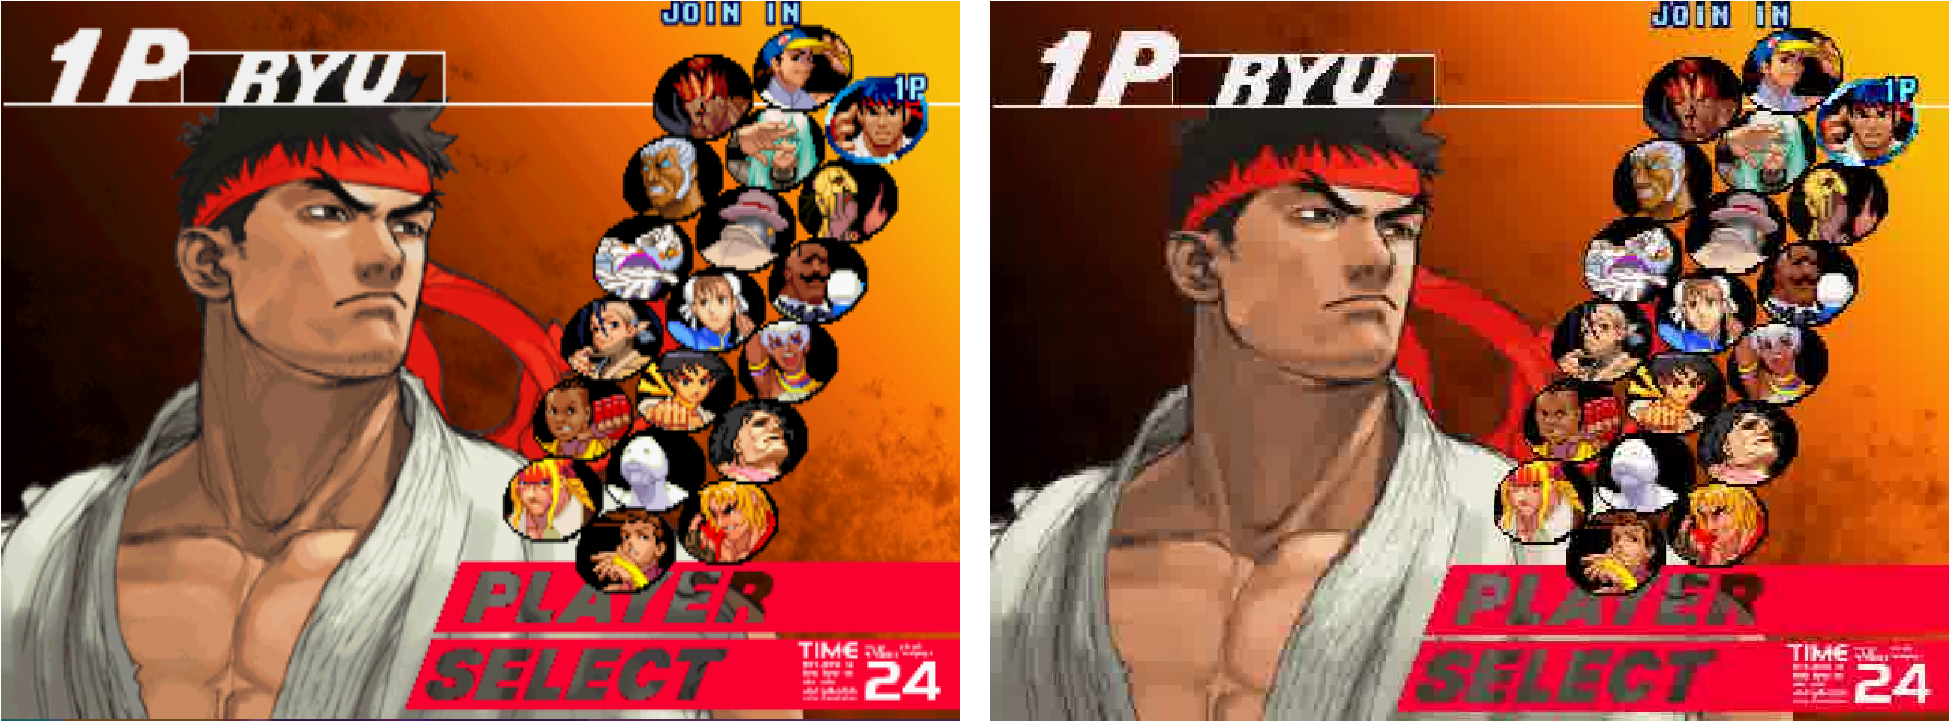
\includegraphics[width=\linewidth]{immagini/ssf3_compare}
	\caption{Comparazione tra rendering e streaming}
	\label{fig:ssf3_compare}
\end{figure}

Lorem ipsum dolor sit amet, consectetur adipiscing elit, sed do eiusmod tempor incididunt ut labore et dolore magna aliqua. Ut enim ad minim veniam, quis nostrud exercitation ullamco laboris nisi ut aliquip ex ea commodo consequat. Duis aute irure dolor in reprehenderit in voluptate velit esse cillum dolore eu fugiat nulla pariatur. Excepteur sint occaecat cupidatat non proident, sunt in culpa qui officia deserunt mollit anim id est laborum.

Lorem ipsum dolor sit amet, consectetur adipiscing elit, sed do eiusmod tempor incididunt ut labore et dolore magna aliqua. Ut enim ad minim veniam, quis nostrud exercitation ullamco laboris nisi ut aliquip ex ea commodo consequat. Duis aute irure dolor in reprehenderit in voluptate velit esse cillum dolore eu fugiat nulla pariatur. Excepteur sint occaecat cupidatat non proident, sunt in culpa qui officia deserunt mollit anim id est laborum.

Lorem ipsum dolor sit amet, consectetur adipiscing elit, sed do eiusmod tempor incididunt ut labore et dolore magna aliqua. Ut enim ad minim veniam, quis nostrud exercitation ullamco laboris nisi ut aliquip ex ea commodo consequat. Duis aute irure dolor in reprehenderit in voluptate velit esse cillum dolore eu fugiat nulla pariatur. Excepteur sint occaecat cupidatat non proident, sunt in culpa qui officia deserunt mollit anim id est laborum.

\begin{figure}[H]
	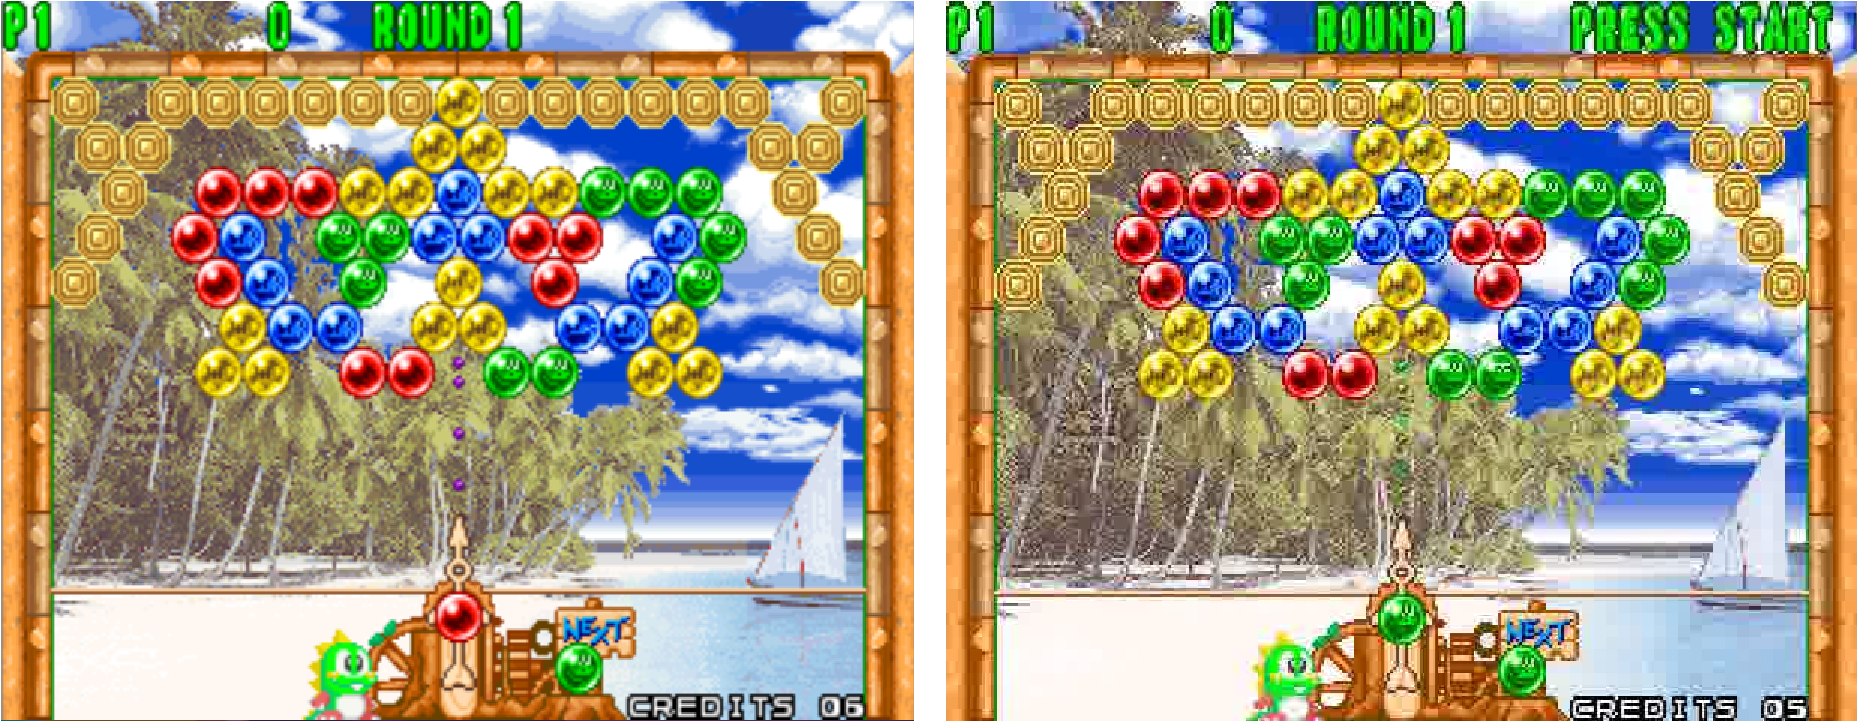
\includegraphics[width=\linewidth]{immagini/puzzle_compare}
	\caption{Comparazione tra rendering e streaming}
	\label{fig:puzzle_compare}
\end{figure}

Lorem ipsum dolor sit amet, consectetur adipiscing elit, sed do eiusmod tempor incididunt ut labore et dolore magna aliqua. Ut enim ad minim veniam, quis nostrud exercitation ullamco laboris nisi ut aliquip ex ea commodo consequat. Duis aute irure dolor in reprehenderit in voluptate velit esse cillum dolore eu fugiat nulla pariatur. Excepteur sint occaecat cupidatat non proident, sunt in culpa qui officia deserunt mollit anim id est laborum.



\section{Larghezza di banda}
Lorem ipsum dolor sit amet, consectetur adipiscing elit, sed do eiusmod tempor incididunt ut labore et dolore magna aliqua. Ut enim ad minim veniam, quis nostrud exercitation ullamco laboris nisi ut aliquip ex ea commodo consequat. Duis aute irure dolor in reprehenderit in voluptate velit esse cillum dolore eu fugiat nulla pariatur. Excepteur sint occaecat cupidatat non proident, sunt in culpa qui officia deserunt mollit anim id est laborum.

Lorem ipsum dolor sit amet, consectetur adipiscing elit, sed do eiusmod tempor incididunt ut labore et dolore magna aliqua. Ut enim ad minim veniam, quis nostrud exercitation ullamco laboris nisi ut aliquip ex ea commodo consequat. Duis aute irure dolor in reprehenderit in voluptate velit esse cillum dolore eu fugiat nulla pariatur. Excepteur sint occaecat cupidatat non proident, sunt in culpa qui officia deserunt mollit anim id est laborum.

Lorem ipsum dolor sit amet, consectetur adipiscing elit, sed do eiusmod tempor incididunt ut labore et dolore magna aliqua. Ut enim ad minim veniam, quis nostrud exercitation ullamco laboris nisi ut aliquip ex ea commodo consequat. Duis aute irure dolor in reprehenderit in voluptate velit esse cillum dolore eu fugiat nulla pariatur. Excepteur sint occaecat cupidatat non proident, sunt in culpa qui officia deserunt mollit anim id est laborum.



\section{Latenza}
Per quanto riguarda la latenza è un problema che non può essere eliminato nel cloud gaming perché le fasi di un videogioco sono: ricezione input, esecuzione, rendering, display; mentre nel caso del cloud gaming si aggiungono: invio al server dell'input utente, codifica audio-video, invio all'utente dello stream video, decodifica audio-video. Un leggero ritardo in un filmato su internet o in una videochiamata molto probabilmente passa inosservato, ma durante una partita la latenza può rendere il gioco ingiocabile, una tempistica di esempio è visibile in Fig. \ref{fig:latenzaCloudGaming}, fortunatamente il rapido sviluppo delle reti a banda larga hanno reso questo problema meno evidente e il cloud gaming una realtà.

\begin{figure}[H]
	\includegraphics[width=\linewidth]{immagini/latenzaCloudGaming.png}
	\caption{Latenza del videogioco: locale vs cloud gaming. Fonte: shadow.tech/blog/news/roadmap-cloud-gaming-without-latency}
	\label{fig:latenzaCloudGaming}
\end{figure}
%license:BSD-3-Clause
%copyright-holders:Michele Maione
%============================================================
%
%	Piattaforma di cloud gaming per giochi arcade
%
%============================================================

\chapter*{Direzioni future di ricerca e conclusioni}
\addcontentsline{toc}{chapter}{Direzioni future di ricerca e conclusioni}

%Si mostrano le prospettive future di ricerca nell'area dove si è svolto il lavoro. Talvolta questa sezione può essere l'ultima sottosezione della precedente. Nelle conclusioni si deve richiamare l'area, lo scopo della tesi, cosa è stato fatto, come si valuta quello che si è fatto e si enfatizzano le prospettive future per mostrare come andare avanti nell'area di studio.

Durante la realizzazione di questo progetto, molte persone dopo aver verificato il funzionamento hanno chiesto quando sarebbe stato reso pubblico; tale richiesta evidenza il grande interesse che hanno ancora oggi i videogiochi arcade per le persone di tutte le età. Il \textit{MAME CGP} si prefiggeva lo scopo di rendere fruibili nel modo più semplice possibile e per la maggior parte dei dispositivi i videogiochi arcade, scopo che si è concretizzato sottoforma di piattaforma di cloud gaming. Credo fermamente che il rilascio del codice sorgente del \textit{MAME CGP} stimolerà altri sviluppatori ad una maggiore innovazione sui sistemi di cloud gaming e sulle tecnologie di streaming in generale, nonché ad ampliamenti del progetto.

Il progetto apre le porte a molte idee e miglioramenti che possono portarlo ad essere effettivamente competitivo. Molto utile per la fidelizzazione dell'utente sarebbe la creazione di un sistema di account tramite cui il giocatore può salvare e caricare lo stato del gioco, pubblicare i punteggi nella leaderboard, invitare altri giocatori ad unirsi alla partita supportando così il multiplayer da devices differenti. Per ridurre la dimensione dei pacchetti si potrebbero usare due codec open-source che in futuro saranno supportati nativamente dalla maggior parte dei browser: \textit{AOMedia Video 1 (AV1)}, progettato per trasmissioni video su Internet, e \textit{Opus}, un codec audio lossy utilizzato per la comunicazione in tempo reale. Ambedue inseribili nel contenitore \textit{WebM}. Per diminuire l'overhead di comunicazione si potrebbe sostituire il protocollo \textit{WebSocket} con \textit{RTP} utilizzabile tramite la tecnologia \textit{WebRTC}. Nella sua versione attuale il progetto è in ascolto su una porta specifica e può essere distribuito su più server utilizzando un software per il bilanciamento del carico (ad esempio \textit{Nginx}), oppure ampliando la classe che si occupa di orchestrare la comunicazione con il client, sfruttando lo stesso protocollo utilizzato per la ricezione dell'input utente si possono scambiare informazioni con altre instanze del \textit{MAME CGP} in esecuzione su altri server per un'efficiente bilanciamento del carico. Un'altra strategia di ottimizzazione, sebbene complessa, consiste nel dividere le varie fasi del cloud gaming in componenti e distribuirle dinamicamente su più server in base alle risorse richieste e disponibili.

A valle di tutto quello di cui si è parlato finora si ritiene che gli obiettivi iniziali della tesi siano stati raggiunti e che il \textit{MAME CGP} è in grado di fungere da piattaforma di cloud gaming. Infine, il fatto che gli sviluppi possibili siano molteplici induce a pensare che il sistema abbia ampi margini evolutivi.

\appendix
\newpage
\pagenumbering{roman}
\setcounter{page}{\thesavepage}

\chapter{Documentazione del progetto logico}
Documentazione del progetto logico dove si documenta il progetto logico del sistema e se è il caso si mostra la progettazione in grande del SW e dell’HW. Quest’appendice mostra l’architettura logica implementativa (nella Sezione 4 c’era la descrizione, qui ci vanno gli schemi a blocchi e i diagrammi).
%\chapter{Documentazione della programmazione}
Documentazione della programmazione in piccolo dove si mostra la struttura ed eventualmente l’albero di Jackson.
\chapter{Listato} \label{chap:Listato}
In questa appendice sono riportate alcune parti del codice C++ a cui si fa riferimento nel testo. Per ogni listato è riportato il file da cui è stato estratto.

\section{Modifiche classi SDL}
Di seguito le modifiche che sono state apportate alle classi originali del MAME nel main e per recuperare il rendering e il missaggio audio.

\subsection{Main}
File \verb|osd/sdl/sdlmain.cpp|

\begin{lstlisting}
int main(int argc, char** argv)
{
	auto r = 0;	
	streaming_server::instance().activate(argc, argv);

	if (streaming_server::instance().is_active())
	{
		streaming_server::instance().on_accept = [&](auto parameters)
		{
			streaming_server::run_new_process(argc, argv);

			r = main_sdl(argc, argv, parameters["game"]);
		};

		streaming_server::instance().start(8888);
	}
	else
		r = main_sdl(argc, argv, "");	

	return r;
}
\end{lstlisting}


\subsection{Missaggio audio} \label{lst:sdl_sound}
File \verb|osd/modules/sound/sdl_sound.cpp|

\begin{lstlisting}
void sound_sdl::sdl_callback(
	void* userdata, Uint8* stream, int len)
{
	//... CODICE NON MODIFICATO ...

	if (streaming_server::instance().is_active())
	{
		streaming_server::instance().send_audio_interval(
			stream, len, this_->sdl_xfer_samples);

		memset(stream, 0, len); //silence local outputs
	}

	//... CODICE NON MODIFICATO ...
}
\end{lstlisting}

\subsection{Rendering}
Files \verb|osd/modules/render/draw13.cpp| e \verb|osd/modules/render/draw13.h|

\begin{lstlisting}[label={lst:draw13}]
void renderer_sdl2::free_streaming_render() const
{
	if (m_sdl_buffer_bytes != nullptr)
	{
		SDL_RWclose(m_sdl_buffer);
		SDL_FreeSurface(m_sdl_surface);
		SDL_DestroyRenderer(m_sdl_renderer);

		delete[] m_sdl_buffer_bytes;
	}
}

void renderer_sdl2::init_streaming_render(
	const int w, const int h, const int fps)
{
	free_streaming_render();

	m_sdl_buffer_bytes_length = w * h * 4;
	m_sdl_buffer_bytes = new char[m_sdl_buffer_bytes_length];

	m_sdl_surface = SDL_CreateRGBSurfaceWithFormat(
		0, w, h, 32, SDL_PIXELFORMAT_RGBA32);

	//Crea il rendering su superfice al posto di quello su finestra
	m_sdl_renderer = SDL_CreateSoftwareRenderer(
		m_sdl_surface);

	m_sdl_buffer = SDL_RWFromMem(
		m_sdl_buffer_bytes, m_sdl_buffer_bytes_length);

	if (streaming_server::instance().is_active())
		streaming_server::instance().init_encoding(w, h, fps);
}

int renderer_sdl2::create()
{
	//... CODICE NON MODIFICATO ...

	if (streaming_server::instance().is_active())
	{
		const auto nd = win->get_size();
		init_streaming_render(
			nd.width(), nd.height(), win->m_win_config.refresh);
	}
	else
	{
		if (video_config.waitvsync)
			m_sdl_renderer = SDL_CreateRenderer(
				dynamic_pointer_cast<sdl_window_info>(
					win)->platform_window(), 
					-1, SDL_RENDERER_PRESENTVSYNC | 
					SDL_RENDERER_ACCELERATED);
		else
			m_sdl_renderer = SDL_CreateRenderer(
				dynamic_pointer_cast<sdl_window_info>(
					win)->platform_window(), 
					-1, SDL_RENDERER_ACCELERATED);
	}

	//... CODICE NON MODIFICATO ...
}

int renderer_sdl2::draw(int update)
{
	//... CODICE NON MODIFICATO ...
	SDL_RenderPresent(m_sdl_renderer);

	if (streaming_server::instance().is_active())
	{
		streaming_server::instance().send_video_frame(
			static_cast<uint8_t*>(m_sdl_surface->pixels));
		SDL_RWseek(m_sdl_buffer, 0, RW_SEEK_SET);
	}
	return 0;
}
\end{lstlisting}

\subsection{Gestione input}
Files \verb|osd/modules/input/input_sdl.cpp|

\begin{lstlisting}
sdl_keyboard_device(
		running_machine &machine, const char *name,
		const char *id, input_module &module): 
	sdl_device(machine, name, id, DEVICE_CLASS_KEYBOARD, module),
	keyboard({{0}})
{
	streaming_server::instance().set_keyboard(this);
}
\end{lstlisting}

\section{Moduli nuovi}
Di seguito alcune funzioni nei due moduli che sono stati creati: codifica e server per la comunicazione WebSocket.


\subsection{Codifica}
File \verb|lib/util/encoding/encode_to_movie.hpp|

\begin{lstlisting}
static int write_packet(
	void* opaque, uint8_t* buf, int buf_size)
{
	auto* const this_ = 
		static_cast<encode_to_movie*>(opaque);

	this_->socket->write(
		reinterpret_cast<const char*>(buf), buf_size);

	return 1; //1 element wrote
}

//Add video frame
void add_frame(const uint8_t* pixels)
{
	if (!header)
		write_header();

	avpicture_fill(
		reinterpret_cast<AVPicture*>(rgb_frame),
		pixels, PIXEL_FORMAT_IN, width, height);
	
	//RGB to YUV
	sws_scale(
		encoder_context->video_converter_context,
		rgb_frame->data, rgb_frame->linesize, 0, height,
		yuv_frame->data, yuv_frame->linesize
	);

	av_init_packet(&video_packet);
	video_packet.data = nullptr;
	video_packet.size = 0;

	avcodec_send_frame(
		encoder_context->video_codec_context, yuv_frame);

	const auto got_packet_ptr = 
		avcodec_receive_packet(
			encoder_context->video_codec_context, 
			&video_packet) == 0;

	if (got_packet_ptr)
	{
		const auto ret = 
			av_interleaved_write_frame(
				encoder_context->muxer_context, 
				&video_packet);

		if (ret == 0)
			send_it();
		else
			error("Error while writing video frame", ret);
	}

	av_packet_unref(&video_packet);
}

//Add audio instant
void add_instant(
	const uint8_t* audio_stream, 
	const int audio_stream_size, 
	const int audio_stream_num_samples)
{
	if (!header)
		write_header();

	wav_frame->nb_samples = audio_stream_num_samples;

	auto ret = avcodec_fill_audio_frame(
		wav_frame,
		AUDIO_CHANNELS_IN,
		AUDIO_SAMPLE_FORMAT_IN,
		audio_stream,
		audio_stream_size,
		1); //no-alignment
	if (ret < 0)
		die("Cannot fill audio frame", ret);

	if (convertedData == nullptr)
	{
		ret = av_samples_alloc(
			&convertedData,
			nullptr,
			AUDIO_CHANNELS_OUT,
			aac_frame->nb_samples,
			AUDIO_SAMPLE_FORMAT_OUT,
			0);			
		if (ret < 0)
			die("Could not allocate samples", ret);
	}

	auto outSamples = swr_convert(
		encoder_context->audio_converter_context,
		//output
		nullptr, 0,
		//input
		const_cast<const uint8_t**>(
			wav_frame->data), wav_frame->nb_samples
	);

	if (outSamples < 0)
		die("Could not convert", outSamples);

	for (;;)
	{
		outSamples = swr_get_out_samples(
			encoder_context->audio_converter_context, 0);

		if (outSamples < 
			encoder_context->audio_codec_context->frame_size * 
			encoder_context->audio_codec_context->channels)
			break;

		swr_convert(
			encoder_context->audio_converter_context,
			//output
			&convertedData, aac_frame->nb_samples,
			//input
			nullptr, 0);

		const auto buffer_size = av_samples_get_buffer_size(
			nullptr,
			encoder_context->audio_codec_context->channels,
			aac_frame->nb_samples,
			encoder_context->audio_codec_context->sample_fmt,
			0);

		if (buffer_size < 0)
			die("Invalid buffer size", buffer_size);

		ret = avcodec_fill_audio_frame(
			aac_frame,
			encoder_context->audio_codec_context->channels,
			encoder_context->audio_codec_context->sample_fmt,
			convertedData,
			buffer_size,
			0);

		if (ret < 0)
			die("Could not fill frame", ret);

		av_init_packet(&audio_packet);
		audio_packet.data = nullptr;
		audio_packet.size = 0;

		int got_packet_ptr;

		ret = avcodec_encode_audio2(
			encoder_context->audio_codec_context, 
			&audio_packet, aac_frame, 
			&got_packet_ptr);

		if (ret < 0)
			die("Error encoding audio frame", ret);

		if (got_packet_ptr)
		{
			audio_packet.stream_index = 1;

			ret = av_interleaved_write_frame(
				encoder_context->muxer_context, &audio_packet);

			if (ret == 0)
				send_it();
			else
				error("Error while writing audio frame", ret);
		}

		av_packet_unref(&audio_packet);
	}
}
\end{lstlisting}


\newpage
\subsection{Server}
File \verb|lib/util/streaming_server.hpp|

\begin{lstlisting}
//Invio input utente a SDL
void generate_key_event(
	const char* key, const string& down) const
{
	SDL_Event e;
	e.type = (down == "D" ? SDL_KEYDOWN : SDL_KEYUP);

	e.key.keysym.scancode = 
		SDL_GetScancodeFromName(key);
	
	e.key.keysym.sym = 
		SDL_GetKeyFromScancode(e.key.keysym.scancode);

	keyboard->queue_events(&e, 1);
}

//Singleton
static streaming_server& instance()
{
	static streaming_server instance;
	return instance;
}

void start(const unsigned short port)
{
	server = make_unique<ws_server>();
	server->config.client_mode = true;
	server->config.port = port;
	server->config.timeout_request = 0; //no timeout

	auto& endpoint = server->m_endpoint["/?"];

	endpoint.on_open = [this](auto connection)
	{
		cout
			<< "-Opened connection from "
			<< connection->remote_endpoint_address << ":"
			<< connection->remote_endpoint_port	<< endl;

		game_thread = make_unique<thread>(
			on_accept, connection->parameters);

		game_start_time = chrono::system_clock::now();

		const auto game = connection->parameters["game"];

		cout
			<< "Starting game: " << game
			<< endl;
	};

	endpoint.on_message = [this](auto connection, auto message)
	{
		const auto msg = message->string();
		const auto values = ws_server::split(msg, ":");

		if (values[0] == "ping")
			process_pausing_mechanism();
		else if (values[0] == "key")
			process_key(values);
	};
	
	endpoint.on_error = [](auto connection, auto code)
	{
		cout
			<< "-Error on connection from "
			<< connection->remote_endpoint_address << ":"
			<< connection->remote_endpoint_port	<< endl
			<< ": " << code.message() << endl;
	};

	endpoint.on_close = [this](auto connection, 
		auto status, auto reason)
	{
		const auto game = connection->parameters["game"];
		const auto game_end_time = chrono::system_clock::now();

		const auto game_total_minute_played = 
			chrono::duration_cast<chrono::minutes>(
				game_end_time - game_start_time);		

		cout
			<< "-Closed connection from "
			<< connection->remote_endpoint_address << ":"
			<< connection->remote_endpoint_port	<< endl
			<< ": " << reason << endl;

		cout
			<< game
			<< " played for: " 
			<< game_total_minute_played.count()
			<< "min." << endl;

		machine->schedule_exit();
	};

	cout
		<< "Game streaming server listening on " 
		<< port	<< endl;

	server->start();

	if (game_thread->joinable())
		game_thread->join();
}
\end{lstlisting}
\chapter{Manuale utente}
In questo appendice viene descritta la procedura di configurazione del programma.

\section{Configurazione}

Nella cartella \verb|./roms/| vanno messe tutte le ROM dei giochi che si vuole rendere disponibili.

Nella cartella \verb|./Streaming/HTML/roms/| vanno messe le copertine dei giochi disponibili in formato PNG, della dimensione $222 \times 315px$.

Nel file \verb|./Streaming/HTML/roms/list.txt| vanno messe le informazioni del gioco, nel seguente formato \verb|rom_name;description;other_info| ad esempio:\\ \verb|sfiii3nr1;Street Fighter III: 3rd Strike;Capcom - 1999|.

\section{Esecuzione}

Per avviare il MAME CGP bisogna eseguire il comando\\ \verb|./mame64 -streamingserver -window -video accel -sound sdl -resolution 640x480@30|\\Per Linux e Windows sono forniti nel progetto i due scripts \verb|run.sh| e \verb|run.bat|.
%\chapter{Esempio di impiego}
Un esempio di impiego del sistema realizzato.
%\chapter{Datasheet}
Eventuali Datasheet di riferimento.


\backmatter
\printbibliography[nottype=misc,title={Bibliografia},heading=bibintoc]
\printbibliography[type=misc,title={Sitografia},heading=bibintoc]

\newpage
\listoffigures

\newpage
\listoftables

\newpage
\printindex

\newpage
\pagenumbering{gobble}
%license:BSD-3-Clause
%copyright-holders:Michele Maione
%============================================================
%
%	Piattaforma di cloud gaming per giochi arcade
%
%============================================================

\chapter*{Ringraziamenti 2.0}

Ringrazio tutti coloro che hanno fatto parte del mio percorso di laurea magistrale:\\
La mia famiglia che crede sempre che io possa fare tutto, senza capire che nei miei limiti è sempre una faticaccia.\\
Dino che ha chiuso il buco che avevo nel petto.\\
Laura \& Giulia, Simona, Eleonora, Martina, Greta e tutte le altre ragazze del dipartimento di farmacia. Grazie per aver reso divertenti le giornate di studio. C'era sempre il sole in biblioteca.\\
I giocatori del BawiTeam. Tra lacrime, infortuni, risate e gioie. Che squadra meravigliosa!\\
I miei compagni di corso: Carrarini, Dettori, Iervolino, Lombardi, Bonapace, Paduano, Vannucci, Zhab'yak per i fantastici progetti fatti insieme.\\
Mario, Fede, Nadia, Giorgio, Giovanni e Mariapina per esserci sempre stati (da oltre 20 anni!).\\
Alessandro, Carmen, Claudio, Barbara, Marika, Grazia, Emiliana, Kikka, anche se non ci siamo visti spesso siete stati vicini.\\
I miei parenti di Treviglio che mi hanno aiutato e ospitato. Grazie per il supporto.\\
I professori del dipartimento di informatica. Ho cercato di trarre il massimo dai vostri insegnamenti per poterli poi concretamente utilizzare.\\
Tutti gli altri, anche se non menzionati, siete nel mio cuore.

\vspace*{\fill}

\begin{figure}[H]
	\centering
	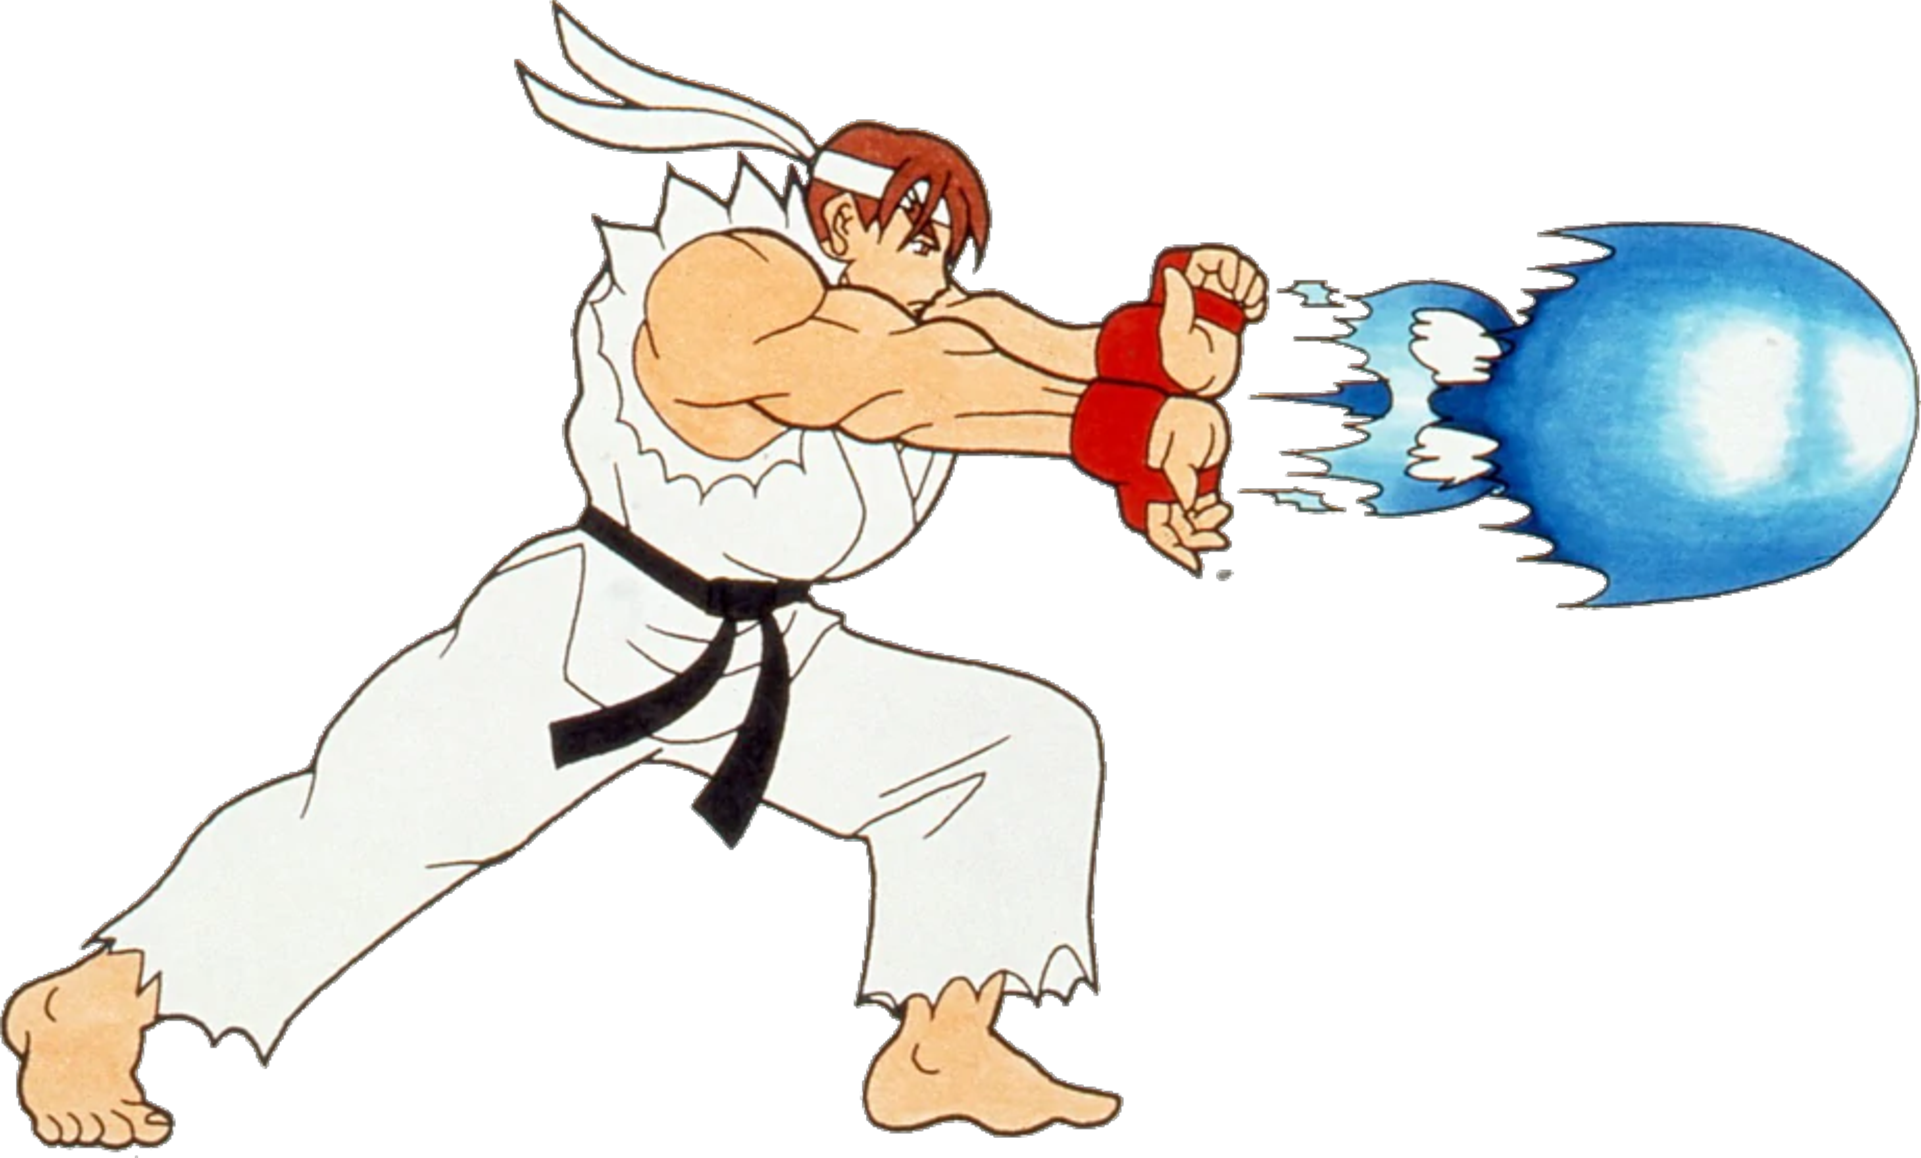
\includegraphics[width=5cm]{immagini/hadoken}
	\caption{Street Fighter Alpha artwork. © Capcom}
	\label{fig:hadoken}
\end{figure}


\end{document}